\documentclass[a4paper]{book}

\usepackage{geometry}
% make full use of A4 papers
\geometry{margin=1.5cm, vmargin={0pt,1cm}}
\setlength{\topmargin}{-1cm}
\setlength{\paperheight}{29.7cm}
\setlength{\textheight}{25.1cm}

% auto adjust the marginals
\usepackage{marginfix}

\usepackage{amsfonts}
\usepackage{amsmath}
\usepackage{amssymb}
\usepackage{amsthm}
%\usepackage{CJKutf8}   % for Chinese characters
\usepackage{ctex}
\usepackage{enumerate}
\usepackage{graphicx}  % for figures
\usepackage{layout}
\usepackage{multicol}  % multiple columns to reduce number of pages
\usepackage{mathrsfs}  
\usepackage{fancyhdr}
\usepackage{subfigure}
\usepackage{tcolorbox}
\usepackage{tikz-cd}
\usepackage{listings}
\usepackage{xcolor} %代码高亮
\usepackage{braket}
\usepackage{algorithm} 
\usepackage{algorithmicx}  
\usepackage{algpseudocode}  
\usepackage{amsmath}  

\floatname{algorithm}{算法}  
\renewcommand{\algorithmicrequire}{\textbf{输入:}}  
\renewcommand{\algorithmicensure}{\textbf{输出:}}  
\renewcommand{\algorithmicrequire}{\textbf{Input : }}
\renewcommand{\algorithmicrequire}{\textbf{Precondition : }}
\renewcommand{\algorithmicensure}{\textbf{Output : }}
\renewcommand{\algorithmicensure}{\textbf{Postcondition : }}
%------------------
% common commands %
%------------------
% differentiation
\newcommand{\gen}[1]{\left\langle #1 \right\rangle}
\newcommand{\dif}{\mathrm{d}}
\newcommand{\difPx}[1]{\frac{\partial #1}{\partial x}}
\newcommand{\difPy}[1]{\frac{\partial #1}{\partial y}}
\newcommand{\Dim}{\mathrm{D}}
\newcommand{\avg}[1]{\left\langle #1 \right\rangle}
\newcommand{\sgn}{\mathrm{sgn}}
\newcommand{\Span}{\mathrm{span}}
\newcommand{\dom}{\mathrm{dom}}
\newcommand{\Arity}{\mathrm{arity}}
\newcommand{\Int}{\mathrm{Int}}
\newcommand{\Ext}{\mathrm{Ext}}
\newcommand{\Cl}{\mathrm{Cl}}
\newcommand{\Fr}{\mathrm{Fr}}
% group is generated by
\newcommand{\grb}[1]{\left\langle #1 \right\rangle}
% rank
\newcommand{\rank}{\mathrm{rank}}
\newcommand{\Iden}{\mathrm{Id}}

% this environment is for solutions of examples and exercises
\newenvironment{solution}%
{\noindent\textbf{Solution.}}%
{\qedhere}
% Define a Solution environment like proof
\makeatletter
\newenvironment{sol}[1][\solname]{\par
  \pushQED{\qed}
  \normalfont \topsep6\p@\@plus6\p@\relax
  \trivlist
  \item[\hskip\labelsep
        \itshape
    #1\@addpunct{.}]\ignorespaces
}{\popQED\endtrivlist\@endpefalse}
\providecommand{\solname}{Solution}
\makeatother
% the following command is for disabling environments
%  so that their contents do not show up in the pdf.
\makeatletter
\newcommand{\voidenvironment}[1]{%
\expandafter\providecommand\csname env@#1@save@env\endcsname{}%
\expandafter\providecommand\csname env@#1@process\endcsname{}%
\@ifundefined{#1}{}{\RenewEnviron{#1}{}}%
}
\makeatother

%---------------------------------------------
% commands specifically for complex analysis %
%---------------------------------------------
% complex conjugate
\newcommand{\ccg}[1]{\overline{#1}}
% the imaginary unit
\newcommand{\ii}{\mathbf{i}}
%\newcommand{\ii}{\boldsymbol{i}}
% the real part
\newcommand{\Rez}{\mathrm{Re}\,}
% the imaginary part
\newcommand{\Imz}{\mathrm{Im}\,}
% punctured complex plane
\newcommand{\pcp}{\mathbb{C}^{\bullet}}
% the principle branch of the logarithm
\newcommand{\Log}{\mathrm{Log}}
% the principle value of a nonzero complex number
\newcommand{\Arg}{\mathrm{Arg}}
\newcommand{\Null}{\mathrm{null}}
\newcommand{\Range}{\mathrm{range}}
\newcommand{\Ker}{\mathrm{ker}}
\newcommand{\Iso}{\mathrm{Iso}}
\newcommand{\Aut}{\mathrm{Aut}}
\newcommand{\ord}{\mathrm{ord}}
\newcommand{\Res}{\mathrm{Res}}
%\newcommand{\GL2R}{\mathrm{GL}(2,\mathbb{R})}
\newcommand{\GL}{\mathrm{GL}}
\newcommand{\SL}{\mathrm{SL}}
\newcommand{\Dist}[2]{\left|{#1}-{#2}\right|}

\newcommand\tbbint{{-\mkern -16mu\int}}
\newcommand\tbint{{\mathchar '26\mkern -14mu\int}}
\newcommand\dbbint{{-\mkern -19mu\int}}
\newcommand\dbint{{\mathchar '26\mkern -18mu\int}}
\newcommand\bint{
{\mathchoice{\dbint}{\tbint}{\tbint}{\tbint}}
}
\newcommand\bbint{
{\mathchoice{\dbbint}{\tbbint}{\tbbint}{\tbbint}}
}





%----------------------------------------
% theorem and theorem-like environments %
%----------------------------------------
\numberwithin{equation}{chapter}
\theoremstyle{definition}

\newtheorem{thm}{Theorem}[chapter]
\newtheorem{axm}[thm]{Axiom}
\newtheorem{alg}[thm]{Algorithm}
\newtheorem{asm}[thm]{Assumption}
\newtheorem{defn}[thm]{Definition}
\newtheorem{prop}[thm]{Proposition}
\newtheorem{rul}[thm]{Rule}
\newtheorem{coro}[thm]{Corollary}
\newtheorem{lem}[thm]{Lemma}
\newtheorem{exm}{Example}[chapter]
\newtheorem{rem}{Remark}[chapter]
\newtheorem{exc}[exm]{Exercise}
\newtheorem{frm}[thm]{Formula}
\newtheorem{ntn}{Notation}
\newtheorem{pro}{Problem}

% for complying with the convention in the textbook
\newtheorem{rmk}[thm]{Remark}


%----------------------
% the end of preamble %
%----------------------

\begin{document}

%\tableofcontents
%\clearpage

\pagestyle{fancy}
%\lhead{Qinghai Zhang}
%\chead{Notes on Algebraic Topology}
%\rhead{Fall 2018}


\setcounter{chapter}{0}


% each chapter is factored into a separate file.

\chapter{2022年上海疫情数据数值拟合}

\pagenumbering{arabic}
\setcounter{page}{1}
\section{introduction}
在已有部分数据的条件下,使用数值方法对现实问题进行模拟预测是
数值科学在现实生活中的常见应用。今年三月以来,上海市疫情爆发引起
社会各界的广泛关注。虽然目前疫情已经基本得到有效控制,但是本文以学习
为目的使用数值方法对疫情数据进行模拟。

本报告中,基于表\ref{fig:numbers}的数据,使用最小二乘拟合和基于
传染病模型SIR方程组的数值求解对
上海疫情以来的数据进行数值模拟。由于
确诊感染数与无症状感染数差距过于悬殊,该文全部数据
取自百度实时确诊/治愈数据。
\begin{table}[H]
  \centering
  \begin{tabular}[H]{|c|c|c|c|c|c|c|c|c|c|c|c|}
    \hline
    日期      & 3.17 & 3.24 & 3.31 & 4.7 & 4.14   & 4.21  & 4.28 & 5.5 & 5.12 & 5.19 & 5.26  \\
    \hline
    累计确诊 & 4944 & 5135 & 6452 & 9334 & 20244 & 39643 & 56300 & 60113 & 61741 & 62521 & 62911  \\
    \hline
    累计治愈 & 4281 & 4779 & 4998 & 5270 & 7936 & 15836 & 31782 & 50871 & 56424 & 58539 & 60499  \\
    \hline
  \end{tabular}
  \caption{上海疫情无症状感染人数统计}
  \label{fig:numbers}
\end{table}

\section{数值模拟}
\subsection{最小二乘拟合}
出于各种理论和实践原因,寻求一些高维物体的低维近似是常见的。
这样做我们可以消除错误或忽略不相关的细节,
如从嘈杂的数据中提取信号或趋势,
或将大量数据减少到更易于管理的数量,
或用简单的近似值替换一些复杂的函数。
我们并不期望这样的近似值是准确的,
实际上,在大多数情况下,我们不希望它是准确的,
但我们希望保留一些与原始数据的相似性。
在线性代数术语中,我们希望将向量从高维空间投影到低维子空间。
实现这一点的最常用且计算方便的方法之一是最小二乘法,
我将在本节中使用的方法。

\begin{defn}
  给定点集$(t_i, y_i), i = 1,\ldots, m$。我们希望找到
  一个$n$维向量$x$函数$f(t, x) : \mathbb{R}^{n + 1} 
  \rightarrow \mathbb{R}$满足"最好"地拟合给定数据,"最好"的
  定义维最小二乘意义下:
  \[\min_{x} \sum_{i = 1}^m (y_i - f(t_i, x))^2.\]
  其中线性的表示$f, x$是线性关系,如下所示
  \[ f(t, x) = x_1 + x_2 t + x_3 t^2 + \ldots + x_n t^{n - 1}.\]
\end{defn}

对于真实数据拟合时,转化为求解微分方程组,在matlab中矩阵除法即得结果
$x$。

当$m = 3, 4, 5, 6, 7$的计算结果如图所示
\ref{fig:spline}\ref{fig:fitting}
\begin{figure}
  \centering
  \subfigure[m = 3, 4 时的最小二乘拟合结果]{
    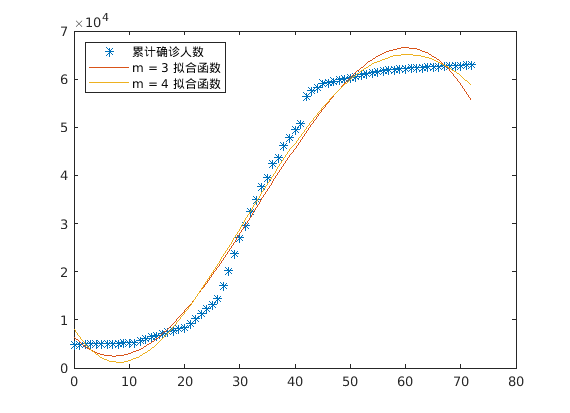
\includegraphics[width=0.43\linewidth]{m34.png}
    \label{fig:spline}}
  \hfill
  \subfigure[m = 5, 6, 7时的最小二乘拟合结果]{
    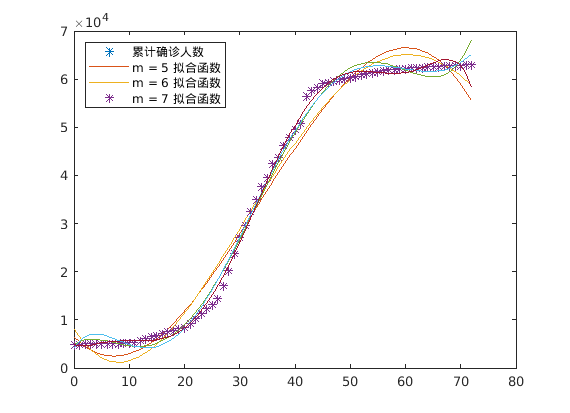
\includegraphics[width=0.43\linewidth]{m567.png}
    \label{fig:fitting}
  }
  \caption{上海无症状感人数拟合结果}
\end{figure}
  从图中可以看出当$m$不够大($m = 3, 4$,左图)时最小二乘拟合结果不理想
  。但是当$m$足够大时继续提升阶数对拟合结果影响不明显(右图),
  并且继续提高$m$会在边界处引起类似拉格朗日龙格现象的震荡如下图
  \ref{mmmm}。对于
  该数据,$m=5$时最合适的拟合阶数。
  \begin{figure}
    \centering
    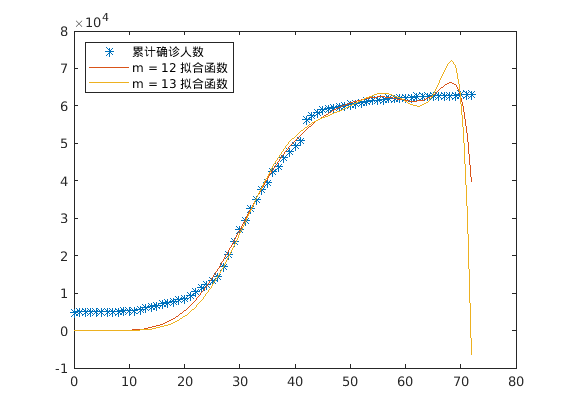
\includegraphics[width=0.43\linewidth]{m1011.png}
    \label{mmmm}
    \caption{当$m$过大时的拟合结果}
  \end{figure}
  
  \section{SIR模型模拟}
  分隔模型是一种非常通用的建模技术。
  它们通常用于传染病的数学建模。
  所有人被分配到带有标签的人群,
  例如S、I或R(易感、感染或恢复)。
  人可能会在人群之间变化。
  标签的顺序通常显示人群之间的流动模式;
  例如,SIR意味着易感,感染,恢复。

  SIR模型最简单的传染病模型之一,很多更深的模型从中衍生发展,
  这个模型分为三个部分,$S(t)$表示易感人群的人数,$I(t)$
  是感染人群人数,$R(t)$是恢复人群。

  通常模型做如下几个假设
  \begin{itemize}
    \item 人口数量始终不变(不考虑人口的出生、死亡和流动等种群动力因素) 
    \[N(t) = S(t) + I(t) + R(t) = N.\]

    \item 一个感染人一旦与易感者接触就会具有一定的传染力,
    假设该传染概率为$\beta$,易感人数减
    少的速度等于转变为感染人数的速度,即
    \[\frac{d S(t)}{dt} = -\beta \frac{I(t)}{N(t)} S(t).\]

    \item 单位时间内从感染者中恢复的人数与感染者数量成正比,以$\gamma$来表示从感染到恢复的比
    例,从而
    \[\frac{d R(t)}{dt} = \gamma I(t).\]
  \end{itemize}
  基于以上这三个假设,我们还可以得到感染人数增加的速度等于易感者增加的速度减去恢复人
数增加的速度,即
 \[\frac{d I(t)}{dt } = \beta \frac{I(t)}{N(t)} S(t) - \gamma I(t).\]

 综上,我们有偏微分方程组 
 \begin{align*}
  \frac{d S(t)}{d t} &= -\beta\frac{I(t)}{N(t)} S(t) \\
  \frac{d I(t)}{d t} &= \beta \frac{I(t)}{N(t)} S(t)-\gamma I(t) \\
  \frac{d R(t)}{d t} &= \gamma I(t),
\end{align*}
初值为$S(0) = 25000000, I(0) = 100, R(0) = 0$.为数值求解该
方程组还需要两个参数值$\beta, \gamma$,采用百度实时疫情动态数据
确诊与治愈人数
$I(t), R(t)$,拟合估算动态$\beta(t), \gamma(t)$,

\begin{figure}
  \centering
  \subfigure[$\beta (t)$]{
    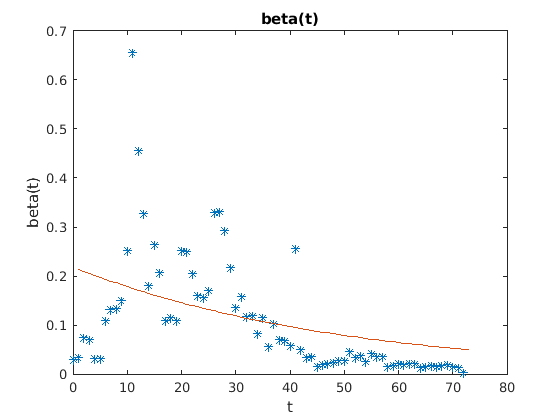
\includegraphics[width=0.43\linewidth]{beta.png}
  }
  \hfill
  \subfigure[$\gamma (t)$]{
    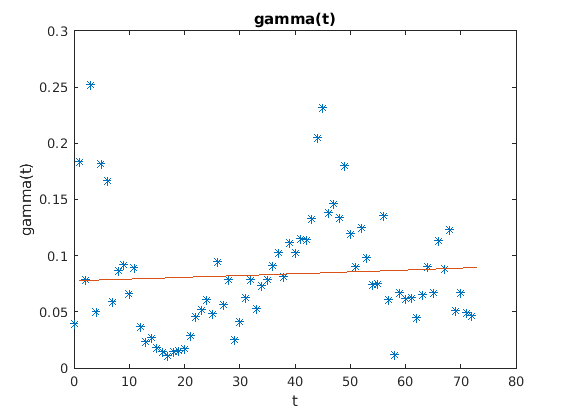
\includegraphics[width=0.43\linewidth]{gamma.png}
  }
  \label{fig:betagamma}
  \caption{参数拟合结果}
\end{figure}
因感染人数相较于上海市常住人口2500万较小,不妨设$N(t) = S(t)$.
可得如图\ref{fig:betagamma}。

\begin{figure}
  \centering
  \subfigure[恢复人数]{
    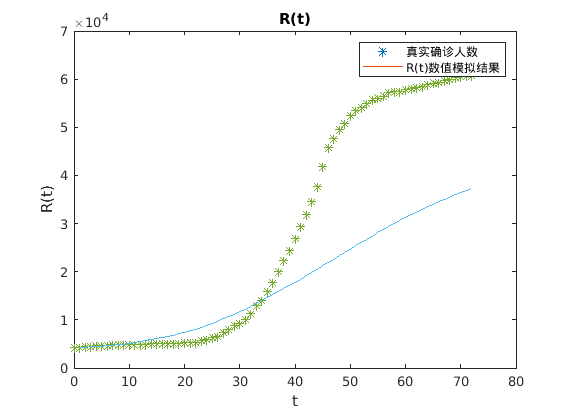
\includegraphics[width=0.43\linewidth]{Rt.png}
  }
  \hfill
  \subfigure[感染人数]{
    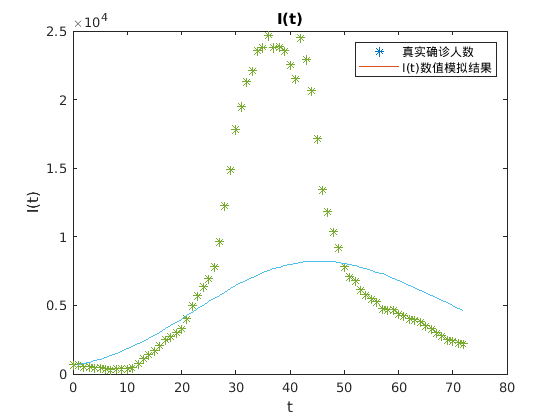
\includegraphics[width=0.43\linewidth]{It.png}
  }
  \label{fig:RIt}
  \caption{参数拟合结果}
\end{figure}
使用matlab自带的龙格库塔步进可得如图\ref{fig:RIt}. 可以看出
结果非常不理想。\ref{fig:betagamma}中拟合$\beta, \gamma$
的源数据分布不佳,可以推断上海疫情数据不适合使用SIR模型进行模拟。

\section{模拟结果分析}
使用最小二乘拟合较为成功的模拟了疫情发展情况,而SIR模型失败了。
我认为原因在于最小二乘没有对疫情发展做过多的相关性假设,导致在
模拟过程中错误的假设对模拟产生负面的影响。

而在SIR模型中,假设了
当感染人群$I(t)$数量上升时对易感人群$S(t)$感染造成线性增长的正相关关系。
虽然在疫情前期缺乏管控期间,理论上确实如此发展,但是在疫情大部分和
主要增长的中后期,政府的防控措施将疫情和绝大部分感染人群$I(t)$
控制在疫区密接人群$M(t)$当中,
该人群数量远小于整个上海的易感人群$M(t) \ll S(t) \approx N(t)$,
因此方程组第一个方程造成了不良影响。另一方面,由于新冠病毒的高
突变概率,恢复人群$R(t)$不能完全避免再度感染,因此第二方程
也不能正确反映感染人群$I(t)$的变化情况。最后,由于在政府管控手段
下恢复人群$R(t)$远没有达到群体免疫的状况下,疫情就接近停息,所以
疫情终止也不是由于SIR模型中的假设的群体免疫。因此综上,SIR较为失败得
拟合上海疫情数据结果是情理之中。

\section{附录}
该节包含两种数值模拟的matlab源代码

\subsection{最小二乘拟合}
\begin{verbatim}
clear
xx = linspace(0,72,73)';
ss = [4944;4964;4986;5027;5066;5080;5094;5135;
    5182;5233;5293;5400;5729;6087;6452;6714;
    7158;7591;7862;8177;8506;9334;10351;11366;
    12283;13281;14471;17044;20244;23838;27078;29498;
    32582;35077;37712;39642;42379;43780;46252;47913;
    49519;50811;56300;57550;58339;59068;59342;59605;
    59868;60113;60366;60583;60907;61141;61370;61514;
    61741;61936;62104;62174;62251;62348;62431;62521;
    62605;62658;62714;62772;62816;62865;62911;62950;
    62982;62988];

cc = [4281;4307;4428;4472;4612;4635;4716;4779;
    4800;4833;4870;4898;4943;4972;4998;5037;
    5068;5098;5125;5166;5213;5270;5389;5616;
    5914;6305;6646;7387;7936;8911;9288;10021;
    11238;12923;14100;15836;17715;19958;22409;24352;
    26992;29302;31782;34593;37649;41891;45873;47742;
    49481;50871;52535;53476;54121;54968;55575;56008;
    56424;57146;57439;57497;57812;58087;58354;58539;
    58798;59142;59379;59759;60027;60371;60499;60661;
    60775;60879];

% yy = ss(2:end) - ss(1:end-1); 
yy = ss(1:end-1);

plot(xx,yy,'*')
% axis([0 72 -30 300])
hold on
dist = 5;
for m=5:1:7
x = xx(1:dist:end);
y = yy(1:dist:end);
A=[];
a=[];
for i=0:1:m
    A = [A x.^i];
end
a = A\y;
u = linspace(0,72)';
f = a(1);
for i=1:1:m
    f = f + a(i+1) * u.^i;
end
plot(u, f,'-');
% plot(u,a(1)+a(2)*u+a(3)*u.^2+a(4)*u.^3 + a(5)*u.^4 + a(6)*u.^5,'-')
hold on
str(m) = "m = " + num2str(m) + " 拟合函数";
end

legend('累计确诊人数', str(5), str(6), str(7) , 'Location', 'NorthWest')
\end{verbatim}

\subsection{SIR数值模拟}
\begin{verbatim}
clear
xx = linspace(0,72,73)';
ss = [4944;4964;4986;5027;5066;5080;5094;5135;
    5182;5233;5293;5400;5729;6087;6452;6714;
    7158;7591;7862;8177;8506;9334;10351;11366;
    12283;13281;14471;17044;20244;23838;27078;29498;
    32582;35077;37712;39642;42379;43780;46252;47913;
    49519;50811;56300;57550;58339;59068;59342;59605;
    59868;60113;60366;60583;60907;61141;61370;61514;
    61741;61936;62104;62174;62251;62348;62431;62521;
    62605;62658;62714;62772;62816;62865;62911;62950;
    62982;62988];

cc = [4281;4307;4428;4472;4612;4635;4716;4779;
    4800;4833;4870;4898;4943;4972;4998;5037;
    5068;5098;5125;5166;5213;5270;5389;5616;
    5914;6305;6646;7387;7936;8911;9288;10021;
    11238;12923;14100;15836;17715;19958;22409;24352;
    26992;29302;31782;34593;37649;41891;45873;47742;
    49481;50871;52535;53476;54121;54968;55575;56008;
    56424;57146;57439;57497;57812;58087;58354;58539;
    58798;59142;59379;59759;60027;60371;60499;60661;
    60775;60879];

I = ss(1:end) - cc(1:end);

dI = I(2:end) - I(1:end-1);
dR = cc(2:end) - cc(1:end-1);

i = I(1:end-1);

gamma = dR ./ i;
beta = (dR + dI) ./ i;

figure(1);
plot(xx, beta, '*'); hold on;
title("beta(t)"); xlabel t; ylabel beta(t);
figure(2);
plot(xx, gamma, '*'); hold on;
title("gamma(t)"); xlabel t; ylabel gamma(t);

syms b(t) g(t)

b = fit(xx, beta,'exp1');
g = fit(xx, gamma, 'exp1');
figure(1); plot(b(xx));
figure(2); plot(g(xx));

f=@(t,y)[y(1)*(b(t)-g(t));g(t)*y(1)];
[x,y]=ode45(f,1:xx(end),[i(1) cc(1)]);

figure(3);
plot(xx, I(1:end-1),'*');
hold on;plot(x,y(:,1));
title("I(t)"); xlabel t; ylabel I(t);
legend('真实确诊人数', "I(t)数值模拟结果");
figure(4);
plot(xx, cc(1:end-1),'*');
hold on;plot(x,y(:,2));
title("R(t)"); xlabel t; ylabel R(t);
legend('真实确诊人数', "R(t)数值模拟结果");
\end{verbatim}

\end{document}
